\documentclass[12pt]{report}
\usepackage[utf8]{inputenc}
\usepackage[english]{babel}
\usepackage[toc,page]{appendix}
\usepackage{microtype}
\usepackage{listings}
\usepackage{blindtext}
\usepackage{graphicx}
\usepackage{xcolor}
\usepackage{bm}
\usepackage{amsmath}
\usepackage{amssymb}
\usepackage{braket}
\usepackage{algorithm,algpseudocode}
\graphicspath{ {images/} }

\DeclareMathOperator*{\argmax}{arg\,max}
\DeclareMathOperator*{\argmin}{arg\,min}

\title{
{Working Title}\\
{\Large University of Oslo}\\
{
\includegraphics{uio.pdf}}
}
\author{Andreas Godø Lefdalsnes}
\date{\today}

\usepackage[backend=bibtex]{biblatex}
\addbibresource{references.bib}

\definecolor{light-gray}{gray}{0.90}

\lstset{basicstyle=\linespread{1.1}\ttfamily\footnotesize,
    keywordstyle=\ttfamily,
    keepspaces=true,
    columns=fixed,
    tabsize=4,
    backgroundcolor=\color{light-gray},
    xleftmargin=0.7cm,
    frame=tlbr, 
    framesep=0.2cm, 
    framerule=0pt,
    frame=single,
    breaklines=true,
}

\begin{document}

\maketitle

\chapter*{Abstract}
Abstract goes here \parencite[e.g.][page 300]{einstein}.
 
\tableofcontents

\chapter{Introduction}
Intro.

\subsection{Molecular dynamics}

\subsection{Atom-centered descriptors}

\subsection{Goals}

\subsection{Contributions}

\subsection{Structure}


\part{Theory}
 
\chapter{Quantum Mechanics}
The discussion in this chapter follows closely the discussion in
[Sakurai | Modern Quantum Mechanics].
\newline
In quantum mechanics, a physical state is represented by a textit{state vector}
in a complex vector space. Such a vector is called a \textit{ket}, denoted
by $\ket{\alpha}$. The state ket is postulated to contain all information
about the physical state. Two kets can be added to produce a new ket:
$$ \ket{\alpha} + \ket{\beta} = \ket{\gamma} .$$
They can also be multiplied by a complex number:
$$ c\ket{\alpha} = \ket{\alpha}c = \ket{\delta} .$$
If $c$ is zero the resulting ket is called a \textit{null ket}.
If $c$ is non-zero it is postulated that the resulting ket contains
the same information.
\newline
Observables such as momentum and spin are represented by operators
acting on the vector space in question. Operators
act on a ket from the left to produce a new ket:
$$ A \ket{\alpha} = \ket{\delta} .$$
Of particular importance is when the action of an operator
on a ket is the same multiplication:
$$ A \ket{\alpha} = c\ket{\alpha} = \ket{\delta} .$$
These kets are known as \textit{eigenkets} and the corresponding
complex numbers are known as \textit{eigenvalues}.
The physical state represented by an eigenket is known
as an \textit{eigenstate}. Any ket
can be written as an expansion of eigenkets $\ket{a'}$:
$$ \ket{\alpha} = \sum_{a'} c_{a'} \ket{a'} ,$$
where $c_{a'}$ is a complex coefficient. In principle
there are infinitely many linearly indepedent eigenkets,
depending on the dimensionality of the vector space.
The uniqueness of the expansion can be proven
with orthonogality of the eigenkets, which we will simply postulate.
\par
A \textit{bra space} is a vector space "dual" to the ket space.
We postulate that for every ket $\ket{\alpha}$ there exists a bra
$\bra{\alpha}$. The bra space is spanned by eigenbras $\bra{a'}$
corresponding to the eigenkets $\ket{a'}$. The ket and bra spaces
have a dual correspondence:


\chapter{Manybody Quantum Mechanics}
This chapter will give a brief overview of the Hartree-Fock
and Density Functional Theory methods, which are the primary workhorses
in manybody quantum theory.
\par
In most applications of quantum theory we are interested in
finding solutions to the non-relativistic time-independent
Schrodinger equation:

$$ \hat{H} \ket{\Psi} = E \ket{\Psi} ,$$

with the Hamiltonian $\hat{H}$ describing a system of nuclei and electrons
with coordinates $\bm{R}_i, \ i=1,2,\dots,A$ and $\bm{r}_i, \
i=1,2,\dots,N$ respectively. The distance between nuclei $a$
and electron $i$ is given as $r_{ai} = \left| \bm{R}_a - \bm{r}_i \right|$
and correspondingly for the nuclei-nuclei and electron-electron distances.
\par
The full Hamiltonian for a set of $N$ electrons and $A$ nuclei
in atomic units is

\begin{equation}
    \begin{split}
        \hat{H} 
        &= -\sum_{i=1}^N \frac{1}{2} \nabla_i^2
        -\sum_{a=1}^A \frac{1}{M_a} \nabla_a^2
        -\sum_{i=1}^N \sum_{a=1}^A \frac{Z_a}{r_{ia}} \\
        &+ \sum_{i=1}^N \sum_{j=i+1}^N \frac{1}{r_{ij}}
        + \sum_{a=1}^A \sum_{b=a+1}^A \frac{Z_a Z_b}{R_{ab}}
    \end{split} .
\end{equation}

The first two terms describe the kinetic energy operators
of the electrons and nuclei, with $M_a$ the ratio of the mass
of nuclei $a$ to the electron mass. The third term describes the
coulomb attraction between electron and nuclei, while the fourth and fifth
terms describe the repulsion between electrons and nuclei respectively.
\par
From this description we are most often interested in the electronic
structure problem presented by applying the \textit{Born-Oppenheimer}
approximation. Since the nuclei are approximately 2000 times heavier
than the electrons, the electrons can to a good approximation
be described as moving in the field of fixed nuclei. This means we
can neglect the kinetic energy terms of the nuclei, while considering
an averaged effect from the nuclei-nuclei repulsion.
The nuclei-nuclei repulsion energy adds a constant to the energy
eigenvalues, but has no effect on the energy eigenfunctions.
The remaining terms are known as the electronic Hamiltonian:

\begin{equation}
    \hat{H}_e = -\sum_{i=1}^N \frac{1}{2} \nabla_i^2
    -\sum_{i=1}^N \sum_{a=1}^A \frac{Z_A}{r_{ia}}
    +\sum_{i=1}^N \sum_{j=i+1}^N \frac{1}{r_{ij}} .
\end{equation}

The electronic wavefunction $\Psi_e = \Psi_e(\{r_i\}; \{R_a\})$
is a function of the electronic coordinates with a parametric dependence
on the fixed nucleic coordinates. The electronic energy
is obtained in the usual way $E_{e} = \braket{\Psi_e | \hat{H}_e |
\Psi_e} $. The total energy of our system
must now include the constant nuclear repulsion:

$$ E_{tot} = E_{e} + \sum_{a=1}^A \sum_{b=a+1}^A
    \frac{Z_a Z_b}{R_{ab}} . $$

If one has solved the Schrodinger equation for the electronic
Hamiltonian, one can subsequently solve for the nucleic motion
using the same method, i.e. substituting the electronic coordinates
for their average values, averaged over the electronic wave function.
We are then left with a nuclear Hamiltonian $\hat{H}_n$:

\begin{equation}
    \begin{split}
        \hat{H}_n 
        &= -\sum_{a=1}^A \frac{1}{2 M_a} \nabla_a^2
        + \langle -\sum_{i=1}^N \frac{1}{2} \nabla_i^2
        - \sum_{i=1}^N \sum_{j=i+1}^N \frac{1}{r_{ij}}
        \rangle \\
        &+ \sum_{a=1}^A \sum_{b=a+1}^A
        \frac{Z_a Z_b}{R_{ab}} \\
        &= -\sum_{a=1}^A \frac{1}{2 M_a} \nabla_a^2
        + E_{tot} .
    \end{split}
\end{equation}

Under this approximation the nuclei move on a potential energy
surface obtained by solving the electronic Hamiltonian.
\par
Finally, we would also like to go one step further and neglect
the relative positions of the nuclei. To this end we consider only the
center of mass of the nucleus with a total charge $Z$,
which gives us the final expression we want for our Hamiltonian:

\begin{equation}
    \hat{H} = -\sum_{i=1}^N \frac{1}{2} \nabla_i^2
    - \sum_{i=1}^N \frac{Z}{r_{i}} + \sum_{i=1}^N \sum_{j=i+1}^N
    \frac{1}{r_{ij}}
\end{equation}

\subsection{Hartree-Fock}
[cite](http://vergil.chemistry.gatech.edu/notes/hf-intro/node3.html)
The Hartree-Fock method is a method for finding
solutions to the electronic Hamiltonian assuming
the electron-electron repulsion can be approximated
with a set of single-particle functions or \textit{orbitals}
moving in a mean field generated by the presence of other electrons.
Assuming that the electrons do not interact
the Hamiltonian is separable and the wavefunction
is simply a product of orbitals $\psi$
which are solutions to a onebody Hamiltonian.
This gives us an ansatz for the manybody wavefunction $\Psi$
known as the \textit{Hartree product}:

$$ \Psi(\bm{r}_1,\dots,\bm{r}_N) = \psi(\bm{r}_1) \cdot \dots
    \cdot \psi(\bm{r}_N) . $$

Since we are dealing with fermions this ansatz fails to satisfy
the antisymmetry principle, i.e. the wavefunction
is not antisymmetric with respect to the interchange of any two
particles. Fermions in addition to three spatial degrees of freedom
also have a spin degree of freedom $\sigma$
which means the fermion can be described
by the space-spin coordinate $\bm{x} = (\bm{r}, \sigma)$
with $\bm{x} \in \mathbb{R}^3 \otimes \sigma$.
\par
The problem of antisymmetry in a system of $N$ fermions
is satisfied by the introduction of \textit{Slater determinants}

\begin{equation}
\Psi(\bm{x}_1,\dots,\bm{x}_N)
= \frac{1}{\sqrt{N}}
\begin{vmatrix}
    \chi_{1}(\bm{x}_1) & \chi_{2}(\bm{x}_1)
    & \dots & \chi_{N}(\bm{x}_1) \\
    \chi_{1}(\bm{x}_2)  & \chi_{2}(\bm{x}_2)
    & \dots & \chi_{N}(\bm{x}_2) \\
    \hdotsfor{4} \\
    \chi_{1}(\bm{x}_N) & \chi_{2}(\bm{x}_N)
    & \dots & \chi_{N}(\bm{x}_N)
\end{vmatrix} ,
\end{equation}

with $\chi(\bm{x})$ spin orbitals and a normalization factor
$(N!)^{-1/2}$. The introduction of this ansatz is equivalent to assuming that
all electrons move independently of each other
in a mean field generated by the electron-electron repulsion.
\par
Define the one-electron operator of the electronic Hamiltonian as

$$ \hat{h}_1(\bm{x}_i) = -\frac{1}{2} \nabla_i^2
    -\frac{Z}{r_i} , $$

with a twobody interaction term

$$ \hat{v}(\bm{x}_i, \bm{x}_j) = \frac{1}{r_{ij}} , $$

with the electronic Hamiltonian written more compactly as

$$ \hat{H} = \sum_i \hat{h}_1(\bm{x}_i)
    + \sum_{i < j} \hat{v}(\bm{x}_i, \bm{x}_j) .$$

The expectation value of the energy is given as

$$ \braket{\Psi | \hat{H} | \Psi} .$$

The \textit{variational theorem} says the expectation
value of any normalized wavefunction with respect to the energy
is an upper bound to the ground state energy.
This suggests a procedure wherein we vary the parameters
of a set of approximate wavefunction $\Psi_T$
until an energy minimum is reached.
\par
The Hartree-Fock energy can be written in terms of integrals
over the onebody and interaction terms:

$$ E_{HF} = \sum_i \braket{i | \hat{h} | i}
    + \sum_{i < j} \braket{ij | \hat{v} | ij}_{AS} ,$$

where we have introduced an antisymmetrized matrix element

$$ \braket{ij | \hat{v} | ij}_{AS}
    = \braket{ij | \hat{v} | ij} - \braket{ij | \hat{v} | ji} , $$

and the shorthand integrals

$$ \braket{i | \hat{h}_1 | i} =
    \int d\bm{r} \chi_i^* \hat{h}_1 \chi , $$

and

$$ \braket{ij | \hat{v} ij} =
    \int d\bm{r}_i d\bm{r}_j \chi_i^* \chi_j^* \hat{v}
    \chi_i \chi_j . $$

In order to solve these integrals numerically
we perform a linear expansion of the spin orbitals
$\chi$ in terms of a fixed orthogonal basis $\phi$:

$$ \chi_i = \sum_{\lambda} C_{i\lambda} \phi_{\lambda} , $$

in principle an infinite sum, but in practice truncated.
\par
This allows us to rewrite the Hartree-Fock energy as

$$ E_{HF} = \sum_i \sum_{\alpha, \beta}
    C_{i \alpha}^* C_{i\beta} \braket{\alpha | \hat{h}_1 | \beta}
    + \sum_{i < j} \sum_{\alpha, \beta, \delta, \eta}
    C_{i\alpha}^* C_{j\beta}^* C_{i\delta} C_{j\eta}
    \braket{\alpha \beta | \hat{v} | \delta \eta} .$$

Work out the remainder here...

\subsection{Density functional theory}
Density functional theory is a method for
investigating the electronic structure of a manybody system
by finding approximations to the ground state
density $\rho(\bm{r})$. Our starting point
is again the electronic Hamiltonian

\begin{equation}
    \hat{H} = -\sum_{i=1}^N \frac{1}{2} \nabla_i^2
    - \sum_{i=1}^N \frac{Z}{r_{i}} + \sum_{i=1}^N \sum_{j=i+1}^N
    \frac{1}{r_{ij}} .
\end{equation}

Any electronic wavefunction $\Psi$ which solves this equation
is in principle a function of $4N$ coordinates $\bm{x}_i = (\bm{r}_i, \sigma_i)
, \ i=1,\dots,N$
where $N$ is the number of electrons.
Once we have obtained a solution to the Schrodinger equation
we can obtain the one-electron density $\rho(\bm{r})$ as:

\begin{equation}
    \rho(\bm{r}) = \int \left| \Psi(\bm{r}, \sigma, \bm{x}_2,\dots,\bm{x}_N)
    \right|^2 d\sigma d\bm{x}_2 \dots d\bm{x}_N .
\end{equation}

Since the wavefunction is a unique functional of the Hamiltonian
$\hat{H}$, the one-electron density is uniquely determined
by the Hamiltonian. Hohenberg and Kohn showed in 1964 in their
first theorem that this mapping
can be inverted, i.e. that the one-electron density uniquely
determines the Hamiltonian of our system (up to an arbitrary constant).
Taken altogether, this means that all properties of our system, including
the Hamiltonian and the manybody wavefunction are fixed
by a one-electron density carrying a dependency on only 3 spatial coordinates.
\par
The electronic Hamiltonian can be rewritten as

$$ \hat{H} = \hat{F} + \hat{V}_{ne} , $$

where $\hat{F}$ is an operator consisting of the kinetic energy
and electron-electron operators and $\hat{V}_{ne}$
is the electron-nuclei interaction.
\par
For their second theorem, Hohenberg and Kohn defined
the universal density functional

$$ F[n] = \braket{\Psi[n] | \hat{F} | \Psi[n]} , $$

and the total electronic energy functional

$$ E[n] = F[n] + \int \hat{V}_{ne} n(\bm{r}) d\bm{r} . $$

Hohenberg and Kohn showed the energy functional
with respect to $N$-electron densitites $n(\bm{r})$
is an upper bound to the ground state energy:

$$ E_0 \leq F[n] + \int \hat{V}_{ne} n(\bm{r}) d\bm{r} , $$

with equality if and only if the one-electron density
is the one-electron density corresponding to our system $\hat{H}$.
This suggests a variational procedure, wherein
we minimize the total electronic energy functional
until we reach an energy minimum:

$$ E_{min} = \underset{n}{\min} \ E[n] , $$

which serves as our best estimate for the ground state
one-electron density $\rho_0(\bm{r})$.
\par
Levy and Lieb proposed to redefine the universal density functional
in terms of normalized antisymmetric wavefunctions $\Psi$
which yield a fixed density $\rho$:

$$ F[n] = \underset{\min}{\Psi \rightarrow \rho}
    \braket{\Psi | \hat{F} | \Psi}
    = \braket{\Psi[n] | \hat{F} | \Psi[n]} , $$

wherein the minima search is performed over wavefunctions
which yield the fixed density $\rho$.
A search is then performed over densitities $\rho$
until we reach an energy minimum. This method
is known as the \textit{constrained search formulation}.
However, we still do not have an explicit expression
for the universal density functional $F[n]$, and
direct approximations have proved difficult.
\par
Kohn and Sham proposed to decompose $F[n]$ as

$$ F[n] = T_s[n] + E_{Hxc}[n] , $$

where $T_s[n]$ is a non-interacting kinetic-energy functional
which can be defined through the constrained-search formulation:

$$ T_s[n] = \underset{\Phi \rightarrow n}{\min}
    \braket{\Phi | \hat{T} | \Phi}
    = \braket{\Phi[n] | \hat{T} | \Phi[n]} , $$

wherein the minima search is now performed over normalized
single-determinant wavefunctions $\Phi$ which yield
the fixed density $\rho$. The functional
$E_{Hxc}[n]$ is known as the Hartree-exchange-correlation
functional. The variational procedure is then
performed over single-determinant wavefunctions
which yield a fixed density $\rho$ and then
minimized over densities:

\begin{equation}
    \begin{split}
        E_0
        &= \underset{n}{\min} \set{
            F[n] + \int \hat{V}_{ne} n(\bm{r}) d\bm{r} } \\
        &= \underset{n}{\min} \
            \underset{\Phi \rightarrow n}{\min} \set{
            \braket{\Phi | \hat{T} + \hat{V}_{ne} | \Phi}
            + E_{Hxc}[n_{\Phi}]} \\
        &=  \underset{\Phi}{\min}
            \set{ \braket{\Psi|\hat{T} + \hat{V}_{ne}|\Phi}
            + E_{Hxc}[n_{\Phi}]} .
    \end{split}
\end{equation}

As with the Hartree-Fock method, the single determinant
wavefunctions are constructed from an orthonormal basis of spin orbitals
$\chi_i (\bm{x}), \ i=1,\dots,N$ with $\bm{x} = (\bm{r}, \sigma)$.
The total electronic energy can be expressed in terms of spatial
orbitals $\phi_i(\bm{r})$ after integrating over the spin variables:

\begin{equation}
    E = \sum_i \int \phi_i^* (\bm{r}) (-\frac{1}{2} \nabla^2 + \hat{v}_{ne})
        \phi_i(\bm{r}) d\bm{r} + E_{Hxc}[n] ,
\end{equation}

with the density expressed as

\begin{equation}
    n(\bm{r}) = \sum_i \left| \phi_i(\bm{r}) \right|^2 .
\end{equation}

With the constraint that the spatial orbitals be normalized
we obtain the following Lagrangian:

$$ \mathcal{L} [\set{\phi_i}]
    = E[\set{\phi_i}] - \sum_i \epsilon_i
    \left( \int \phi_i^* (\bm{r}) \phi_i(\bm{r}) d\bm{r} - 1 \right) , $$

with $\epsilon_i$ the associated Lagrangian multiplier.
We find the energy minimum where the Lagrangian is stationary:

$$ \frac{\partial \mathcal{L}}{\partial \phi_i^* (\bm{r})} = 0 . $$

The spatial orbitals are expanded as a linear combination
of a known basis, such as hydrogen-like functions
or Gaussian-type orbitals:

$$ \phi_i(\bm{r}) = \sum_{\lambda} C_{\lambda i} \chi_i (\bm{r}) . $$

 
\chapter{Molecular Dynamics}
From quantum mechanics to molecular dynamics.

\subsection{Molecular dynamics simulations}

\subsection{Molecular dynamics potentials}

 
\chapter{Machine learning}
Machine learning is the study of algorithms and statistical models employed by computing systems
capable of performing tasks without explicit instruction. While traditional algorithms
rely on some specified input and a ruleset for determining the output, machine learning
is instead concerned with a set of generic algorithms which can find patterns
in a broad class of data sets. This section will give a brief overview of machine learning,
and more specifically the class of algorithms known as neural networks, and will follow closely the review by
% cite here
[Mehta et. al.] which the reader is encouraged to seek out.
\par
Examples of machine learning problems include identifying objects in images,
transcribing text from audio and making film recommendations to viewers based on their watch history.
Machine learning problems are often subdivided into estimation and prediction problems.
In both cases, we choose some observable $\bm{x}$ (e.g. the period of a pendulum)
related to some parameters $\bm{\theta}$ (e.g. the length and the gravitational constant)
through a model $p(\bm{x} \lvert \bm{\theta})$ that describes the probability of observing
$\bm{x}$ given $\bm{\theta}$. Subsequently we perform an experiment to obtain a dataset
$\bm{X}$ and use these data to fit the model. Fitting the model means finding
the parameters $\hat{\bm{\theta}}$ that provide the best explanation for the data. 
\textit{Estimation} problems are concerned with the accuracy of $\hat{\bm{\theta}}$, whereas
prediction problems are concerned with the ability of the model $p(\bm{x} \lvert \bm{\theta})$
to make new predictions.
Physics has traditionally been more concerned with the estimation of model parameters, while in
this thesis we will be focused on the accuracy of the model.
\par
Many problems in machine learning are defined by the same set of ingredients.
The first is the dataset $\mathcal{D} = (\bm{X}, \bm{Y})$, where $\bm{X}$ is a matrix
containing observations of the independent variables $\bm{x}$, and $\bm{Y}$ is a matrix containing
observations of dependent variables. Second is a model $\bm{F}: \bm{x} \rightarrow \bm{y}$
which is a function of the parameters $\bm{\theta}$. Finally we have a cost function
$\mathcal{C}\left(\bm{Y}, \bm{F}\left(\bm{X} ; \bm{\theta}\right)\right)$
that judges the performance of our model at generating predictions.
\newline
In the case of linear regression we consider a set of independent observations
$ \bm{X} = 
\begin{bmatrix}
\bm{x}_1 & \bm{x}_2 & \dots & \bm{x}_N
\end{bmatrix}
$
related to a set of dependent observations $\bm{y} = (y_1, y_2, \dots,y_N)$
through a linear model 
%\newline
$f(\bm{x} ; \bm{\theta}) = 
x_1\cdot w_1 + x_2\cdot w_2 + \dots + x_P\cdot w_P$,
with parameters $\bm{\theta} = (w_1, w_2, \dots,w_P)$. The cost function
is the well known sum of least squares $\mathcal{C}(\bm{y}, f(\bm{X} ; \bm{\theta}))
= \sum_i^N (y_i - f(\bm{x}_i ; \bm{\theta}))^2 $ and the best fit is chosen as the set
of parameters which minimize this cost function: $\hat{\bm{\theta}} = \underset{\bm{\theta}}
{\text{argmin}} \ \mathcal{C}(\bm{Y}, f(\bm{X} ; \bm{\theta})) $.

\subsection{Basics of statistical learning}
% needs revision
Statistical learning theory is a field of statistics dealing with the problem
of making predictions from data. We begin with an unknown function \newline
$y = f(x)$ and our goal is to develop a function $h(x)$
such that $h \sim f$. We fix a hypothesis set $\mathcal{H}$ that the
algorithm is willing to consider. The expected error of a particular $h$
over all possible inputs $x$ and outputs $y$ is:
$$ E[h] = \int_{X \times Y} \mathcal{C}(h(x), y) \rho(x,y) dx dy ,$$
where $\mathcal{C}$ is a cost function and $\rho(x,y)$ is the joint probability
distribution for $x$ and $y$. This is known as the \textit{expected error}.
Since this is impossible to compute without knowledge of the probability distribution
$\rho$, we instead turn to the \textit{empirical error}. Given $n$ data points
the empirical error is given as:
$$ E_S[h] = \frac{1}{n} \sum_i^n \mathcal{C}(h(x_i), y_i) .$$
The \textit{generalization error} is defined as the difference
between the expected and empirical errors:
$$ G = E[h] - E_S[h] .$$
We say an algorithm is able to learn from data or \textit{generalize} if 
$$ \lim_{n\to\infty} G = 0 .$$

We are in general unable to compute the expected error, and therefore unable
to compute the generalization error. The most common approach known as
\textit{cross-validation} is to estimate the
generalization error by subdividing our dataset into a \textit{training} set
and a \textit{test} set. The value of the cost function on the training set
is called the \textit{in-sample} error and the value of the cost
function on the test set the \textit{out-of-sample} error.
Assuming the dataset is sufficiently large and representative of $f$, and the subsampling
into train and test datasets is unbiased, the in-sample error
can serve as an appropriate proxy for the generalization error.
\newline
In figure \ref{fig:in-out}
we show the typical evolution of the errors as the number of data points increase.
It is assumed that the function being learned is sufficiently complicated
that we cannot learn it exactly, and that we have a sizeable number of data points
available. The in-sample error will decrease monotonically, as our model
is not able to learn the underlying data exactly. In contrast, the out-of-sample
error will decrease, as the sampling noise decreases and the training
data set becomes more representative of the underlying probability distribution.
In the limit, these errors both approach same value, which is known the model
\textit{bias}. The bias represents the best our model could do in the infinite data limit.
The out-of-sample error produced from the sampling noise
is known as \textit{variance}, and will vanish completely
given an infinite representative data set.

% create own figures or cite properly
\begin{figure}[h]
    \centering
    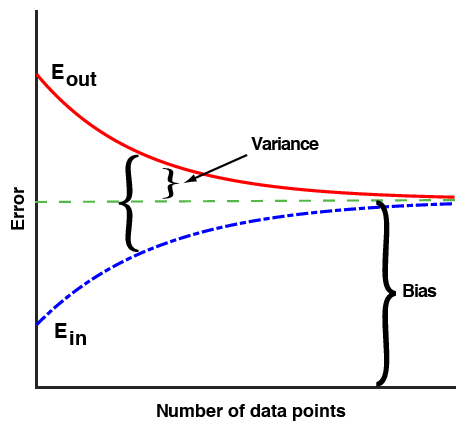
\includegraphics[width=0.75\linewidth]{in-out-sample.png}
    \caption{Typical in-sample and out-of-sample error as a function
    of the number of data points. It is assumed that the number
    of data points is not small, and that the true function
    cannot be exactly fit.}
    \label{fig:in-out}
\end{figure}

In figure \ref{fig:bias-variance} we show the typical evolution
of the out-of-sample error as the model \textit{complexity} increases.
Model complexity is a measure of the degrees of freedom in the model space,
for example the number of coefficients in a polynomial regression.
In the figure we can see that bias decreases monotonically as model complexity
increases, as the model is able to fit a larger space of functions.
However, the variance will also increase as the model becomes more
susceptible to sampling noise. In general the lowest out-of-sample error,
and therefore generalization error, is achieved at an intermediate
model complexity. We also find that as model complexity increases,
a larger amount of data points is required to be able to reasonably
fit the true function.

% create own figures or cite properly
\begin{figure}[h]
    \centering
    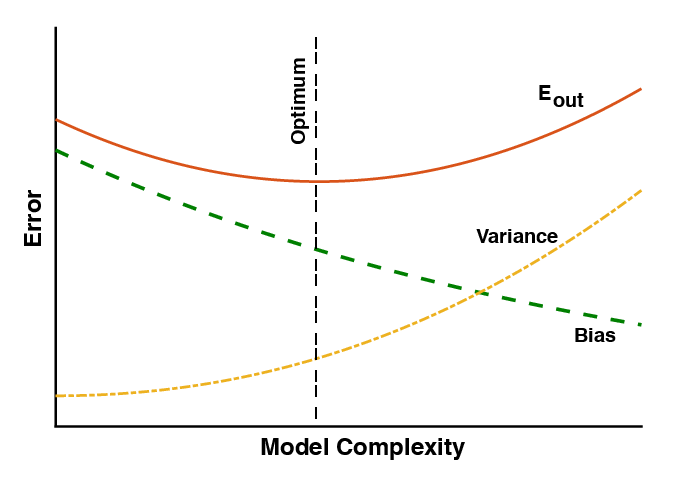
\includegraphics[width=0.75\linewidth]{bias-variance.png}
    \caption{Typical out-of-sample error as a function
    of model complexity for a fixed dataset. Bias decreases monotonically with
    model complexity, while variance increases as a result of
    sampling noise.}
    \label{fig:bias-variance}
\end{figure}

\subsection{Bias-variance decomposition}
Consider a dataset $\mathcal{D}(\bm{X}, \bm{y})$ of $n$ pairs
of independent and dependent variables. Assume the true data
is generated from a noisy model:
$$ y = f(\bm{x}) + \epsilon ,$$
where $\epsilon$ is normally distributed with mean $\mu$ and
standard deviation $\sigma$. Assume that we have an estimator $h(\bm{x}; \bm{\theta})$
trained by minimizing a cost function $\mathcal{C}(\bm{y}, h(\bm{x}))$
which we take to be the sum of squared errors:
$$ \mathcal{C}(\bm{y}, h(\bm{x})) = \sum_i^n (y_i - h(\bm{x}_i; \bm{\theta}))^2 .$$
Our best estimate for the model parameters:
$$ \bm{\theta}_{\mathcal{D}} = \underset{\bm{\theta}}{\argmin} \
\mathcal{C}(\bm{y}, h(\bm{x}; \bm{\theta})) ,$$
is a function of the dataset $\mathcal{D}$. If we imagine we have a set of
datasets $\mathcal{D}_j = (\bm{y}_j, \bm{X}_j)$, each with $n$ samples, we would like to calculate
the expectation value of the cost function over all these datasets $E_{\mathcal{D}, \epsilon}$.
We would also like to calculate the expectation value over different instances of the noise $\epsilon$.
The expected generalization error can be decomposed as:
% more in depth?
\begin{equation}
\begin{split}
    E_{\mathcal{D}, \epsilon} [\mathcal{C}(\bm{y}, h(\bm{X} ; \bm{\theta}_{\mathcal{D}}))]
    &= E \left[ \sum_i (y_i - h(\bm{x}_i ; \bm{\theta}_{\mathcal{D}}))^2 \right] \\
    &= \sum_i \sigma_{\epsilon}^2 + E_{\mathcal{D}}[(f(\bm{x}_i) - f(\bm{x}_i ; \bm{\theta}_{\mathcal{D}}))^2] .
\end{split}
\end{equation}

The second term can be further decomposed as
\begin{equation}
\begin{split}
    &E_{\mathcal{D}}[(f(\bm{x}_i) - f(\bm{x}_i ; \bm{\theta}_{\mathcal{D}}))^2] \\
    &= (f(\bm{x}_i) - E_{\mathcal{D}}[h(\bm{x}_i ; \bm{\theta}_{\mathcal{D}})])^2
    + E[(h(\bm{x}_i ; \bm{\theta}_{\mathcal{D}}) - E[h(\bm{x}_i ; \bm{\theta}_{\mathcal{D}}])^2]
\end{split}
\end{equation}

The first term is what we have referred to as the bias:

\begin{equation}
    \text{Bias}^2 = \sum_i (f(\bm{x}_i) - E_{\mathcal{D}}[h(\bm{x}_i ; \bm{\theta}_{\mathcal{D}})])^2.
\end{equation}

The bias measures the expectation value of the deviation of our model from the true
function, i.e. the best we can do in the infinite data limit.
\newline
The second term is what we have referred to as the variance:
\begin{equation}
    \text{Var} = \sum_i  E[(h(\bm{x}_i ; \bm{\theta}_{\mathcal{D}}) - E[h(\bm{x}_i ; \bm{\theta}_{\mathcal{D}}])^2]
\end{equation}

The variance measures the deviation of our model due to finite-sampling effects.
Combining these effects we can decompose the out-of-sample error into:
\begin{equation}
    E_{\text{out}} = \text{Bias}^2 + \text{Var} + \text{Noise},
\end{equation}

with $\text{Noise} = \sum_i \sigma_{\epsilon}^2$.
\newline
In general it can be much more difficult to obtain sufficient good data
than to train a very complex model. Therefore it is often useful in practice
to use a less complex model with higher bias, because it is less susceptible
to finite-sampling effects.

\subsection{Neural networks}
Artificial Neural Networks (ANN) or Deep Neural Networks (DNN) are
supervised learning models vaguely inspired by biological neural networks.
The building blocks of neural networks are neurons that take a
vector input of $d$ features $\bm{x} = (x_1,\dots,x_d)$
and produce a scalar output $a(\bm{x})$.
A neural networks consists of layers of these neurons stacked together
with the output of one layer serving as input for another. The
first layer is typically known as the \textit{input layer}, the
middle layers as \textit{hidden layers} and the final layer
the \textit{output layer}. The basic architecture is shown in
figure \ref{fig:neural-networks}.
In almost all cases the output $a_i(\bm{x})$ of neuron $i$ can be decomposed
into a linear operation on the inputs passed through a non-linear
activation function:
$$ a_i(\bm{x}) = \sigma_i(z_i) ,$$
where $\sigma_i$ is a non-linear function and $z_i$
is the dot product between the inputs $\bm{x}$ and a set of
neuron-specific weights $\bm{w}_i$:
$$ z_i = \bm{x}^T \bm{w}_i + b_i .$$
The term $b_i$ is a neuron-specific re-centering of the input.
\newline
Typical choices of non-linearities/activation functions include
the sigmoid and hyperbolic tangent functions, and Rectified Linear Units (ReLU).
When the activation function is non-linear, the neural network with a single hidden
layer can be proven to be a \textit{universal function approximator},
given an arbitrarily large number of neurons. We typically also
want functions that are monotonic and smooth with a monotonic derivative.
\newline

% own figure or cite
\begin{figure}[h]
    \centering
    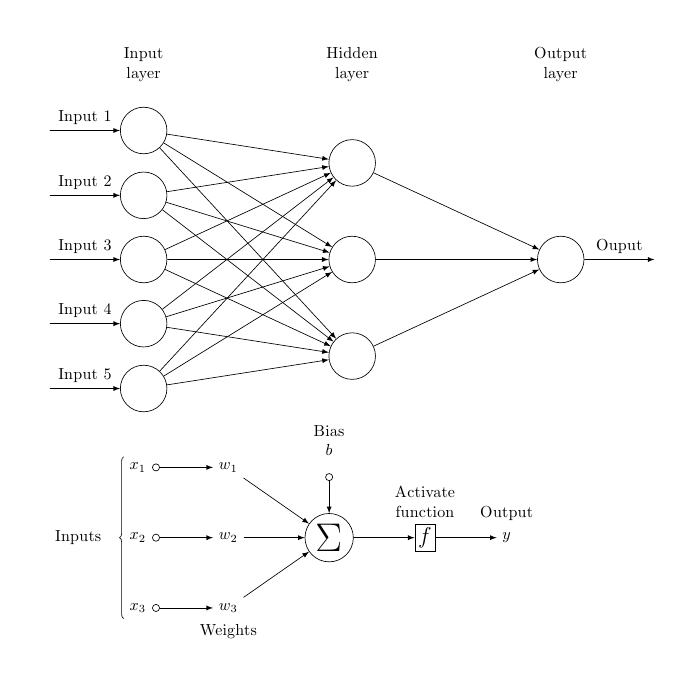
\includegraphics[width=0.75\linewidth]{neural-networks.png}
    \caption{Text.}
    \label{fig:neural-networks}
\end{figure}

The simplest neural networks are known as \textit{feed-forward} neural networks (FNN).
The input layer is the vector $\bm{x}$ of inputs, while each neuron in the first
hidden layer performs a dot product between its weights $\bm{w}_i$ and the inputs
and passes it through a non-linearity $\sigma_i$. The activation function
is typically shared across one or multiple layers $\sigma_i = \sigma$. The vector of neuron outputs
$\bm{a}_i$ serves as input to the next hidden layer until we reach the final layer.
In the final layer the choice of activation function is dependent on the problem
we are trying to solve. If we are performing non-linear regression the
final activation function is often the identity $\sigma_i(z) = z$, or if
we are doing classification the soft-max function is often employed.
\newpage
Let $\bm{x}$ be a vector of $d = 1,\dots,D$ inputs or \textit{features}. Let $a_i^{(h)}$
denote the output of neuron $i = 1,\dots,N_d$ in layer $h = 1,\dots,H$.
The output of neuron $i$ in the first hidden layer $a_i^{(1)}$ is thus:
$$ z_i^{(1)} = \bm{x}^T \bm{w}_i^{(1)} + b_i^{(1)} .$$
$$ a_i^{(1)} = \sigma_i^{(1)}(z_i^{(1)}), $$
The inputs are iterated through each hidden layer until we reach the final layer:
$$ z_i^{(H)} = (\bm{a}_{H-1})^T \bm{w}_i^{(H)} + b_i^{(H)} .$$
\begin{equation}
\begin{split}
    a_i^{(H)} &= o_i = \sigma_i^{(H)}(z_i^{(H)}) \\
    &= \sigma_i^{(H)} \left((\bm{a}_{H-1})^T \bm{w}_i^{(H)} + b_i^{(H)} \right) \\
    &= \sigma_i^{(H)} \left(
    \left( (\sigma_1^{(H-1)},\dots,\sigma_{N_{H-1}}^{(H-1)}) \right)^T
    \bm{w}_i^{(H)} + b_i^{(H)} \right) .
\end{split}
\end{equation}

This allows us to compose a complicated function $\bm{F}: \mathbb{R}^D \rightarrow
\mathbb{R}^O$, with $D$ the number of inputs and $O$ the number of outputs.
The \textit{universal approximation theorem} tells us that this simple architecture
can approximate any of a large set of continuous functions
given appropriate choice of weights $\bm{w}_i^h$ and mild assumptions
on the activation functions. The theorem requires only a single hidden layer,
where the strength of the approximation relies on the number of neurons.
In practice it has been found that adding more layers produces
faster convergence and higher accuracy, which has given rise
to the field of \textit{deep learning}.

\subsection{Backpropagation}
Text.

\subsection{Optimization}
More text.


\chapter{Atom-centered descriptors}
Electronic structure calculations are among the most computationally
intensive scientific calculations, and the rapid development
of modern computers have made many previously unthinkable
computer simulations a central part of the scientific toolkit.
Because of their computationally demanding nature, electronic
structure calculations today occupy a large portion of resources
on modern scientific supercomputer facilities.
\par
For small-scale systems, we have discussed the Hartree-Fock
and Density Functional Theory methods as the primary workhorses
of ab-initio
electronic structure calculations. However, these methods suffer
from very poor scaling as the system size increases, with Hartree-Fock
naively scaling as $\mathcal{O}(N^4)$ with $N$ the number of electrons
and Density Functional Theory scaling as $\mathcal{O}(N^4)$,
but with a larger proportionality scaling.
\par
In many cases the exact details of the electronic structure
are less important than the long-time behaviour of the atoms
and molecules involved in the simulation, and classical approximations
can be made as in molecular dynamics, which comes close
to linear scaling. This allows us to simulate systems
of up to millions or hundreds of millions of atoms,
which can approximate nano- or micro-scale systems if
periodic boundary conditions are applied.
However, the question remains as to how you develop an
accurate classical potential which can accurately reproduce
fundamentally quantum systems, with a speed that allows
us to enter into realistic timescales (i.e. nano or microseconds).
\par
The most common approach to developing molecular dynamics potentials
is to guess a functional form based on your physical intuition
and experience with the systems and calculate appropriate parameters
from data obtained from DFT calculations.
The number of parameters involved can range from two in the case
of Lennard-Jones or hundreds of parameters in the case
of complex, many-atom potentials such as the AMBER and CHARMM
force fields. The imposition of functional forms to quantum data
is an artform, and the potential must often be tailored to not
only the chemical species and number of atoms in your system,
but also the specific experimental quantity you are trying to extract,
such as the energy, radial distribution function or transport
coefficients. Notably there are dozens of MD potentials
describing different models of water (H2O), each fine-tuned
for a specific system structure or parameter.
\newline
\newline
Due to recent developments in the field of machine learning,
the question has been raised as to how it may be possible to
automate the process of developing potentials.
In their article introducing the Atomistic Machine-Learning Package
(AMP) \parencite[Khorshidi, Alireza and Peterson, Andrew A.]
{khorshidi2016amp} outline one potential way forward.
The idea is to approximate the potential energy
with a regression model:

$$ \left\{ \bm{R} \right\} \overset{\text{Regression}}{\longrightarrow}
    E = E\left( \left\{ \bm{R} \right\}\right) , $$

where $\left\{\bm{R}\right\}$ is the set of nuclear coordinates of our system.
Most machine learning methods operate over a set of one-dimensional
so-called \textit{feature vectors}, where every vector element
represents a feature of the data set. For example the amount
of precipation in a given area at a given time is a function
of features such as humidity, cloud cover, air pressure etc.
This is a vector of some length $F$, while the nuclear coordinates
represent a point in $3N$-dimensional phase space.
This difference in representation requires some way of mapping
the nuclear coordinates to features which can be employed
by a machine learning method.
\par
The naive approach would be to simply feed in the nuclear coordinates
as a 1D vector, and then perform a regression on the dataset
in order to obtain the potential energy. However, our physical intuition
imposes some constraints on the potential energy.
In particular, the potential energy of a microscopic system should
be translationally, rotationally and permutationally invariant.
\par
Translational invariance implies that the addition of any
three-dimensional vector to every coordinate in the system should
not in any way alter the potential energy of the system.
This should not be the case with a naive mapping, as for a given
set of weights (or equivalent) smaller/larger coordinates
values would be mapped to smaller/larger activations, and therefore
alter the final output.
Rotational invariance implies that the potential energy
of the system should not change as the system is rotated
about an axis. This also should not be the case in the context
of a naive mapping, as any change to any of the inputs
would be mapped in a non-linear way to produce a different output.
Finally, permutation invariance implies that swapping the coordinates
of any two atoms of the same chemical species would produce the
same potential energy. This should also not be the case, for
the same reasons as we just discussed.
These constraints together heavily restrict the functional form
that any mapping to the potential energy could have,
which means a more careful analysis should be considered.
\newline
\newline
In order for the mapping to be applicable to systems of varying size,
a decomposition into atomic energy contributions is performed:

$$ E(\set{\bm{R}}) = \sum_{i=1}^N E_{\text{atom}}(\set{\bm{R}}) . $$

The individual energy contributions $E_{\text{atom}}$
are then approximated by performing a regression analysis.
The atomic energy contributions are usually limited to its
local environment through the introduction of a cutoff radius $R_c$:

$$ E_{\text{atom}} (\set{\bm{R}}) \approx
    E_{\text{atom}} (\bm{R}_i, \set{\bm{R}_j | \left| \bm{R}_{ij} \right|
    < R_c}) $$

meaning that interactions are only treated if the interatomic distance
is smaller than the cutoff. This is a good approximation for a sensible
choice of cutoff radius if no electrostatic interactions are involved.
Long-range interactions can also be treated through
the introduction of methods such as Ewald summation, but this will
not be discussed here.
\par
A mapping that satisfies the above constraints we will refer to
as a \textit{descriptor}, and is used as input to the regression method:

$$ \set{\bm{R}} \rightarrow \bm{G}(\set{\bm{R}}) \overset{\text{regression}}
    {\longrightarrow} E_{\text{atom}} =
    E_{\text{atom}}(\bm{G}(\set{\bm{R}})). $$

Once we have a descriptor and a regression model the dynamics
can be readily obtained by taking derivatives:

\begin{equation}
\begin{split}
    \bm{F}_i &= -\nabla_i E \\
    &= -\nabla_i \sum_i^{\text{local}}
    E_{\text{atom}}(\bm{G}(\set{\bm{R}})) \\
    &= -\sum_i^{\text{local}} \sum_j \frac{\partial E_{\text{atom}}}
    {\partial G_j} \frac{\partial G_j}{\partial \bm{R}_i} ,
\end{split}
\end{equation}

where we have applied the chain rule to break the gradient
into derivatives with respect to the network inputs (obtained through
backpropagation) and derivatives of the network inputs with
respect to the coordinates of atom $i$.
Once we have the forces the system can be propagated through time
using the Velocity-Verlet equations.

\subsection{Gaussian descriptors}
In their paper on neural-network representations of
potential energy surfaces \parencite[Behler, J\"{o}rg and
Parrinello, Michele]{behler2007generalized}
suggested the decomposition of the mapping $\bm{G}_i$ of atom $i$
into two subvectors $\bm{G}_i^I$ and $\bm{G}_i^{II}$ representing
pairwise and three-body interactions respectively.
The components of $\bm{G}_i^I$ are comprised of
sums of gaussian functions of the pairwise distance $R_{ij}$:

$$ f_i^I = \sum_{j \neq i}^{\text{local}}
    \exp \left( -\eta(R_{ij} - R_s)^2 / R_c^2 \right) f_c (R_{ij}) , $$

with the sum over the local environment of atom $i$.
The parameters $\eta$ and $R_s$ represent the width and center
of the gaussian functions respectively. The term $f_c$
is a cutoff function which decays smoothly to zero
at the cutoff radius. Behler and Parrinello proposed
the following cutoff:

\begin{equation}
    f_c(R) =
\begin{cases}
    \frac{1}{2}\left(1 + \cos \left(\pi R / R_c \right) \right) & R < R_c \\
    0 & R > R_c ,
\end{cases}
\end{equation}

however other functional forms are possible. For the angular part
such terms are multiplied, which means the function decays much more
rapidly as we approach the cutoff. The only requirement we pose
is that the function be continuous with a continuous first derivative
in $r \in [0, \infty)$,
approach one as $R \rightarrow 0$
and zero as $R \rightarrow R_c$.
\par
The components of the three-body subvector are defined incorporating
the angles $\theta_{ijk}$ between every triplet of atoms:

\begin{equation}
\begin{split}
    f_i^{II} &= 2^{1 - \zeta} \sum_{j,k \neq i}^{\text{local}}
    (1 + \lambda \cos \theta_{ijk})^{\zeta}
    \exp \left( -\eta \left( R_{ij}^2 + R_{ik}^2 + R{jk}^2
    \right) / R_c^2 \right) \\
    & \times f_c(R_{ij}) f_c(R_{ik}) f_c(R_{jk}) .
\end{split}
\end{equation}

The components for each subvector is calculated by varying
the different parameters $\eta, R_s, \zeta, \lambda$.
The choice of neither symmetry functions, cutoff, nor the parameters
employed by Behler and Parrinello are unique. The guiding
wisdom is that atomic environments with different
potential energies should give differing energies,
while remaining invariant under translation, rotation and permutation.
Finally we note that the descriptors and the neural network
models are not interchangeable, as each neural network
is trained for a specific set of input vectors, and must
be retrained if the way inputs are composed changes.

% Zernike? Bispectrum?

\subsection{Deep Potential Molecular Dynamics}
Deep Potential Molecular Dynamics (DPMD) is a method
proposed by \parencite[Zhang et al.]{PhysRevLett.120.143001}
in response to the successes of methods such as Behler-Parrinello,
Gaussian Approximation Potentials (GAP)
and Gradient-Domain Machine Learning (GDML).
These methods all involve some amount of handcrafting the inputs,
and building these inputs for larger, more complex systems is not
straightforward.
The Deep Potential method assigns a local environment and reference
frame to each atom. The total potential energy is a sum
of atomic contributions as before:

$$ E = \sum_i E_i , $$

with the atomic energy determined by its nearest neighbors:

$$ E_i = E(\bm{R}_i, \set{\bm{R}_j : \left| \bm{R}_{ij}
    \right| < R_c}) . $$

The position of each neighbor of atom $i$ is described
by the relative positions $\bm{R}_{ij} = \bm{R}_j - \bm{R}_i$,
which preserves translational symmetry.
\par
Rotational symmetry is conserved by constructing a local frame
for each atom. Two neighboring atoms $a$ and $b$ are picked by a
user-specified rule (default: two closest).
The environment of atom $i$ is then described by three unit vectors:

\begin{equation}
\begin{split}
    \bm{e}_{i1} &= \bm{e}(\bm{R}_{ia}) , \\
    \bm{e}_{i2} &= \bm{e}(\bm{R}_{ib} - (\bm{R}_{ib} \cdot \bm{e}_{i1})
    \bm{e}_{i1}) , \\
    \bm{e}_{i3} &= \bm{e}_{i1} \times \bm{e}_{i2} ,
\end{split}
\end{equation}

where $\bm{e}(\bm{R})$ denotes the normalized vector $\bm{e}(\bm{R})
    = \bm{R} / \left| \bm{R} \right|$. Together these vectors
form an orthonormal basis for the reference frame of atom $i$.
The local coordinates $\bm{R}_{ij}$
can then be obtained from the global coordinates $\bm{R}_{ij}^0$
through the transformation:

\begin{equation}
    \bm{R}_{ij} = \bm{R}_{ij}^0 \cdot \mathcal{R} ,
\end{equation}

where $\mathcal{R} = [\bm{e}_{i1} \ \bm{e}_{i2} \ \bm{e}_{i3}]$
is a rotation matrix with columns given by the local basis vectors.
\par
The neural network input vector for every atom-to-atom interaction
$\bm{D}_{ij}$ can be given with radial-only or full radial-angular
information:

\begin{equation}
    D_{ij}^{\alpha} =
\begin{cases}
    \displaystyle\left( \frac{1}{R_{ij}}, \frac{\bm{R}_{ij}}{\left| \bm{R}_{ij} \right|}
    \right) & \text{full information}, \\[10pt]
    \displaystyle\left( \frac{1}{R_{ij}} \right) & \text{radial-only information},
\end{cases}
\end{equation}

with $\alpha = 0$ when only radial information is specified
and $\alpha = 0,1,2,3$ when full information is provided. Radial information
is typically sufficient for long-range interactions such as van-der-Waals
forces, while covalent bonding can be modeled by including
only the closest atoms. We therefore specify two separate
cutoff shells, one for the radial information $R_c$ and one
for treating angular interactions $R_a$.
\par
In order to preserve permutation symmetry the inputs vectors $\bm{D}_{ij}$
are sorted first according to chemical species, and then within
each chemical species according to their inverse distance $1 / R_{ij}$.
The vector of subvectors $\bm{D}_i$ is then fed through a neural
network to produce the atomic energy contribution.
The network input size is fixed according to the maximum number of neighbors
in the system which is being studied, with $\bm{D}_{ij} = \bm{0}$
if there are fewer neighbors within the radial cutoff.
\par
The authors also propose a scheme of force learning, wherein
the force Root Mean Square Error (RMSE) is incorporated into the Loss Function:

\begin{equation}
    \mathcal{L} = \frac{p_{\epsilon}}{N} \sum_i
    \left( \Delta E_i^2 \right)
    + \frac{p_{f}}{3N} \sum_i \left| \Delta \bm{F}_i \right|^2,
\end{equation}

with $p_{\epsilon}$ and $p_{f}$ energy and force pre-factors which are
adjusted throughout the learning process. The term $\Delta E_i$
denotes the error between the sum of network outputs
and the correct potential energy, while the term $\Delta \bm{F}_i$
denotes the error in the force output.
The pre-factors are adjusted based on the learning rate:

\begin{equation}
    p(t) = p^{\text{limit}} \left[ 1 - \frac{r_l(t)}{r_l^0} \right]
    + p^{\text{start}} \left[ \frac{r_l(t)}{r_l^0} \right] ,
\end{equation}

with $r_l(t)$ and $r_l^0$ the learning rate at time step $t$ and time step
$0$ respectively. The learning rate decays exponentially as:

$$ r_l(t) = r_l^0 \cdot d_r^{t / d_s} , $$

with $d_r$ the decay rate and $d_s$ the decay steps. The decay
rate should be less than 1. The force error is often a magnitude or two
larger than the energy error, and it is believed that incorporating
the force into the loss should improve the learning rate for
physics-based applications which incorporate forces.
The virial information can also be treated in this manner,
but this will not be discussed here.


\part{Implementation}
\chapter{Atomic Simulation Environment}
The Atomic Simulation environment (ASE\footnote{
\url{https://wiki.fysik.dtu.dk/ase/index.html}})
\parencite[Larsen et al.]{larsen2017atomic}
is a software package written in Python for the purpose
of setting up, steering and analyzing atomistic simulations.
Python is an interpreted, high-level general purpose language,
with a powerful, consise syntax which allows one to perform
very complex tasks with few lines of code. Python can also
easily be extended and interfaced with fast and mature
libraries. The modular interface of Python makes ASE
easily extensible: in particular the calculator interface
for evaluating energies, forces and much more has been
implemented for software packages such as LAMMPS, VASP,
Quantum Espresso and many more.
The Atomic Simulation Environment is intended to be:

\begin{itemize}
    \item Easy to use
    \item Flexible
    \item Customizable
    \item Pythonic
    \item Open to participation
\end{itemize}

The real drawback of Python is that it is an interpreted language,
which results in slow execution. It can also be quite memory-intensive,
which makes pure Python unsuitable for large scale computations
and simulations. It is therefore common to write the
computationally demanding tasks in a lower level compiled language,
and build a Python interface for calling functions and classes.

\subsection{Installation}
ASE requires an installation of

\begin{itemize}
    \item Python 2.7, 3.4-3.6
    \item Numpy 1.9 or newer
    \item Scipy 0.14 or newer
\end{itemize}

This can be easily obtained through the Anaconda 
or Miniconda packages\footnote{\url{https://anaconda.org/}},
or follow the instructions on the Python website\footnote{
\url{https://www.python.org/}}.
Once you have the prerequisites ASE can be installed using pip:

\begin{lstlisting}[language=bash]
pip install ase
\end{lstlisting}

\subsection{Molecular Dynamics}
Here we will demonstrate how to setup a simple Argon crystal,
set the velocities and integrate the system using
the Velocity Verlet equations.
First we import some prerequisites and define the system:

\begin{lstlisting}[language=python,basicstyle=\small]
from ase.lattice.cubic import FaceCenteredCubic
from ase import units
from ase.md.velocitydistribution import MaxwellBoltzmannDistribution
from ase.md.verlet import VelocityVerlet

symbol = "Ar"
size = (3, 3, 3)
atoms = FaceCenteredCubic(symbol=symbol, size=size, pbc=True)
MaxwellBoltzmannDistribution(atoms, 300 * units.kB)
\end{lstlisting}

This defines a face-centered-cubic (FCC) crystal unit cell
with 4 atoms, and a system size of $3\times3\times3$ unit cells
for a total of $4\cdot3^3 = 108$ atoms with periodic boundary conditions.
We thereafter give the atoms velocities according to the
Maxwell-Boltzmann distribution such that the system temperature
is approximately 300 Kelvin.
\par
Next we give the atoms a Lennard-Jones \textit{calculator}
for calculating dynamics and create a Velocity Verlet \textit{integrator}
for operating on the atoms according to their forces.
Calculators will be discussed in the next section.

\begin{lstlisting}
calc = LennardJones(sigma=3.405, epsilon=1.0318e-2)
atoms.set_calculator(calc)
dyn = VelocityVerlet(atoms, 5 * units.fs)
\end{lstlisting}

The parameters $\sigma$ and $\epsilon$ define the well known
length and energy scales for the Lennard-Jones potential.
The Velocity Verlet integrator is initialized with a timestep
of 5 femtoseconds, which strikes a balance between accuracy
and the timescale of the simulation.
Finally we run the system for 1000 steps:

\begin{lstlisting}
for i in range(100):
    dyn.run(10)
\end{lstlisting}

Every 10 timesteps the system can be printed, written to file
or some other form of analysis and processing.

\subsection{Calculators}
The calculator interface gives ASE an easy to use,
flexible and customizable way of computing dynamics,
and makes ASE viable for a wide range of electronic structure calculations.
For ASE a calculator is a black box that receives positions, atomic
numbers and so on and outputs energies, forces, stresses;
all that is required to perform atomistic simulations.
The basic interface is defined in the ASE source code as:

\begin{lstlisting}[language=python,basicstyle=\small]
import numpy as np


class Calculator:
    def get_potential_energy(self, atoms=None, 
                             force_consistent=False):
        return 0.0

    def get_forces(self, atoms):
        return np.zeros((len(atoms), 3))

    def get_stress(self, atoms):
        return np.zeros(6)

    def calculation_required(self, atoms, quantities):
        return False
\end{lstlisting}

There is also an interface for DFT calculators, which also
requires the implementation of spins, occupation numbers,
the fermi level and so on.
\newline
\newline
In the previous section we used the Lennard-Jones calculator
as an example, however this is generally not advised.
Apart from the Lennard-Jones being a toy potential unsuited
for real systems, the ASE implementation is also written in pure
Python, which makes it very, very slow.
Usually the calculator interface is used as a wrapper for much faster
compiled code or software packages; for example the
Asap calculator is a Python wrapper for the Effective Medium Theory
potential which is implemented in Fortran, and is orders of magnitudes
faster. A Python molecular dynamics code is justified
since the bulk of computation code is spent on computing forces,
however for large scale molecular dynamics simulations
one would be advised to use fast compiled code such as LAMMPS\footnote{
\url{https://lammps.sandia.gov/}} or GROMACS\footnote{
\url{http://www.gromacs.org/}}.
ASE really shines when it comes to small-scale simulations,
experimentation and testing out new methods, and this is why
it has been chosen as a basis for this thesis.
Fortunately, ASE has an extensive code base of calculators
for Molecular Dynamics and Density Functional Theory codes
such as Asap, CP2K, LAMMPS, GROMACS which are all
implemented in lower-level languages.


\chapter{Atomistic Machine-learning Package}

\chapter{Pytorch}

\part{Results}

\chapter{Empirical potentials}

\chapter{Ab-Initio Molecular Dynamics}
 
\chapter{Conclusion}
In this thesis we have trained neural networks to reproduce
molecular dynamics potentials using the Behler-Parrinello method.
These potentials are high-dimensional functions with many parameters
to be determined, and are often developed through intimate knowledge
of the physical and chemical properties of the systems they are designed for.
In addition there are certain symmetries which must be respected when
developing potentials, in particular translational, rotational and permutational
symmetries, as well as conserving energy over time (in the NVE ensemble).
Traditional ab-initio methods suffer from poor scaling as the size of the systems
increases, while classical potentials derived from ab-initio calculations
allows us to simulate realistic scales of up to millions of atoms
depending on the computer resources and the complexity of the atoms in the system.
Since these neural networks when trained offer linear scaling,
they could serve both as supplements to ab-initio methods
or be deployed for calculations using classical molecular dynamics.
For example, one could save many CPU cycles by producing and training
on a small trajectory calculated from DFT, and then use the neural networks
to produce the remainder of the data, provided the neural networks
are reasonably accurate.
While our neural network potential scales linearly with system size,
it has a rather large pre-factor dependent on the symmetry function set,
cutoff radius and the average number of neighbors in the system.
We believe this could be improved by moving more calculations to lower
level compiled languages, such as calculations of neighbor lists,
fingerprints and fingerprint derivatives for every step.
Although we have only ran the neural networks on a single core,
the potential could be parallelized over the atoms
using algorithms such as LAMMPS neighbor lists without
too much overhead.
\par
Unfortunately we were not able to achieve energy conservation
with our neural networks. 
This a central feature of any neural network potential,
and without energy conservation, we cannot sample properties in equilibrium,
as for example the radial distribution function or the diffusion constant
is increasing over time and ill defined.
Generally we find an increase in kinetic energy over time, corresponding
to an increase in potential energy as the atoms move apart,
and an increase in translational momentum.
This indicates holes in the training data from sampling in equilibrium,
as the network seems to perform poorly on unseen configurations with larger
forces, and produce large force residuals.
The results are notably different for the EMT and Stillinger-Weber potential,
this is caused by among other things the symmetry function sets and the
average number of neigbors in the system.
The Stillinger-Weber explicitly includes three-body interactions,
while the EMT potential is a function of interatomic distances, and our
results suggest that the balance between the number of radial and symmetry functions
should be decided by more careful analysis of their relative importance.
\par
On the test trajectory we achieved reasonable values of the energy and force
root mean squared errors, approximately 0.1 eV for the energy and 0.05-0.1 eV/Å
for the force. These are mostly consistent with the results others have achieved
such as \cite{stende2017constructing, treider2017speeding, khorshidi2016amp,
    PhysRevLett.120.143001},
though the energy is often on the order of 1-10 meV, which is lower than
what we have achieved. This is partly due to the fact that we have emphasized
training with forces, which comes at the expense of the energy fit.
Since the training Root Mean Squared Errors (RMSEs) 
is substantially lower than the test RMSE this may
indicate overfitting, though we would not expect this to be a substantial problem
with such a small network with applied regularization.
We note that this has not been tested extensively,
and more testing could produce different results.

\subsection{Prospects and future work}
In this thesis we barely scratched the surface of combining machine learning
methods with molecular dynamics. There are therefore many, many paths
to be explored for future theses or even articles to be published,
which may be achieved working through ASE and/or AMP and making modifications
or writing your own code from scratch. We will list some of the prospects
considered while writing this thesis in semi-ordered order of importance,
though there are likely many which have not been considered.

\begin{itemize}
    \item Numerical optimization:
        In order to speed up the training and deployment of neural
        networks the Atomistic Machine-learning Package (AMP)
        authors created efficient Fortran implementations
        of the Behler-Parrinello symmetry functions.
        This is an improvement over pure Python code, but not enough to
        be satisfied.
        Many parts of the fingerprinting, including neighborlists,
        dictionary data structures, IF tests and so on are currently
        implemented in Python code. This means we are limited in terms
        of CPU time and memory in how fast we can alter hyperparameters
        and train neural networks on new datasets, and how quickly
        the neural networks can be deployed and evaluated in molecular dynamics.
        First and foremost we would suggest moving the calculation of
        the neighborlists, fingerprints and fingerprint derivatives entirely
        to Fortran or some other efficient compiled language.
        This would reduce the speed of evaluations which are currently performed
        in Python, and reduce communication overhead between the Python APIs
        and the Fortran compiled functions.
        For more information see \href{
            https://listserv.brown.edu/cgi-bin/wa?A2=AMP-USERS;d7c6c98c.1904}{
            this post} on the AMP mailing list.
        Once we have our input data and labels, training can be performed
        efficiently using software packages such as Tensorflow or Pytorch,
        and training moved to GPUs with little effort.
    \item Parallelization and LAMMPS:
        As we have discussed in the chapter on the Atomistic Machine-learning Package,
        AMP is planned to provide support for the OpenKIM API which would provide
        the means to export the neural networks to LAMMPS molecular dynamics
        software for deployment.
        If this is implemented (currently unknown) this could significantly speed up
        the deployment and testing of the neural networks, as LAMMPS 
        is an efficient compiled code,
        with efficient algorithms for parallelizing the force evaluations
        over multiple cores.
    \item Improved sampling method:
        We have observed that sampling from molecular dynamics trajectories
        limits us mostly to systems in equilibrium, which limits the
        range of energies and forces observed in the dataset.
        Neural networks perform unexpectedly when encountering unseen data,
        and the training data therefore restricts the generalization
        properties of the network. Improved sampling algorithms to
        sample a wider range of energies and forces out of equilibrium
        would likely improve the long timescale performance of the neural
        network and make the neural network potential more accurate on
        new configurations.
    \item Neural network implementation:
        Currently AMP provides a neural network implementation written
        by the authors, and a Tensorflow 0.11 module compatible only
        with Python 2.7. We would suggest writing a more modern Tensorflow
        interface, using for example the new Tensorflow 2.0 beta,
        in order to take full advantage of these mature neural network
        implementations. This could among other things improve speed,
        more efficient algorithms for initialization and training
        and a large set of helpful functions for training neural networks
        efficiently.
    \item Determining symmetry function sets:
        We have discussed some methods of determining symmetry functions,
        but not in great detail. Generally you want the symmetry functions
        to cover the radial and angular space, while no two symmetry functions
        should be highly correlated. However, we have observed that
        the same general mix of symmetry functions can produce very
        different results. It would be very beneficial if we had an automated
        approach or highly specified approach to determining the numbers of
        and parameters of the symmetry functions for a wide range of
        potential energy surfaces, which would significantly ease the difficulty
        in training and deploying neural networks using the Behler-Parrinello
        method.
   \item Finding minima:
        The AMP package finds minima in the loss function using an
        interface to the scipy.optimize library of functions.
        In this thesis we have only tested with the BFGS optimizer,
        which is the default in AMP, and the one generally favored
        by the authors and other users. However, finding minima in the cost
        function of neural networks is a complicated affair, which has
        been examined in great detail in the literature.
        First and foremost one could test other optimizer available
        through scipy, such as the basin hopping optimizer.
        If an interface to a more mature neural network software package
        such as Tensorflow is 
        implemented it would be easy to test optimizers such as 
        ADAM, SGD, Adagrad and many more \cite{kingma2014adam}.
    \item New descriptors:
        In this thesis we have restricted our interest to the tried and tested
        Behler-Parrinello symmetry functions as the mapping from
        coordinates to inputs. There have since been many suggestions
        on how to fingerprint atomic systems, such as DPMD, SOAP,
        Zernike and Bispectrum descriptors and so forth
        \cite{PhysRevLett.120.143001, bartok2013representing, khorshidi2016amp},
        some of which are discussed in chapter
        \ref{chap:acd}.
        If the forces can be calculated efficiently and accurately
        these descriptors should be evaluated for use in molecular dynamics.
    \item New machine-learning models:
        In this thesis we have only tested neural networks as the
        machine-learning method for regression, due to the
        explosion of interest and application in recent times.
        Neural networks are favorable due to their ability to scale
        well as the data available increases, but if data is limited
        other machine-learning algorithms may be competitive.
        Since we require the calculation of forces for usage
        in molecular dynamics we require the algorithm to have
        continuous derivatives, and a good example is Kernel Ridge
        Regression, which is currently supported in AMP.
    \item Multiple atom types:
        In this thesis we have limited our attention to single-atom
        systems, though AMP provides support for multiple atoms.
        The Behler-Parrinello method is limited in that a neural network
        has to be trained for every type-type interaction, for example
        an O-H interaction must be treated separately. This means that
        fewer potential energy labels are available for training per neural
        network, and creates a combinatorial problem as the number of interactions
        in the system increases. Suggestions have been made to solve this
        problem such as weighted atom-centered symmetry functions (WACSFs\cite{
            gastegger2018wacsf})
        and these could be implemented and evaluated against
        empirical potentials and neural networks trained using the standard
        approach.
    \item Long-range interactions:
        The Behler-Parrinello approach we have deployed is currently
        limited to short-range interactions within a cutoff sphere,
        and this is not sufficient for long-range interactions such
        as the Coulomb interaction. Using methods such as Ewald summation\cite{
            toukmaji1996ewald},
        the Behler-Parrinello method could accommodate this, and this
        would facilitate training on systems containing for example
        water or biological molecules.
\end{itemize}



\begin{appendices}

\chapter{Title 1}

\chapter{Title 2}

\end{appendices}

\printbibliography

\end{document}

